\documentclass[12pt]{article}
\newcommand{\template}{../../../template}
\usepackage{\template/packages}

\newcommand{\titolo}{Appunti di Intelligenza Artificiale}
\newcommand{\autore}{Rosso Carlo}
\newcommand{\data}{A.A. 2023/2024}
\newcommand{\corso}{Intelligenza Artificiale}

\newcommand{\copertina}{
	\begin{titlepage}
		\begin{center}
			\vspace*{3cm}
			\LARGE{\textbf{\titolo}}\\
			\vspace{0.33cm}
			\Large{\textbf{\data}}\\
			\vspace{0.33cm}
			\Large{\autore}\\
		\end{center}
		\thispagestyle{empty}
	\end{titlepage}
}


\begin{document}
\copertina
\tableofcontents
\newpage

\section{Introduzione}

\paragraph{Che cos'è l'intelligenza?}
La capacità di un agenti di affrontare e risolvere con successo situazioni e
problemi nuovi o sconosciuti.\\
I libri di testo classici definiscono l'IA come lo studio di agenti
intelligenti, che percepiscono il loro ambiente e producono azioni volte a
massimizzare la probabilità di successo nel raggiungere i loro scopi.

\paragraph{Intelligenza Artificiale stretta} si riferisce a qualsiasi
intelligenza artificiale in grado di eguagliare o superare un essere umano in un
compito strettamente definito e strutturato.

\paragraph{Intelligenza Artificiale generale} dovrebbe consentire alle macchine
di applicare conoscenze e abilità in diversi contesti anche di tipo nuovo. Si
tratta di un obiettivo non ancora realizzato e non è detto che sia possibile.\\

Lo scopo dell'IA può essere definito come quello di costruire "agenti
intelligenti". In particolare, l'IA studia come riprodurre in un computer 
processi mentali complessi. Questo conduce a due diverse prospettive:
\begin{itemize}
	\item construire dispositivi più intelligenti, che si avvicinano e superano
		l'intelligenza umana (prospettiva ingegneristica);

	\item costruire e testare ipotesi specifiche sui meccanismi all'interno 
		della scatola (cervello), per simulare e studiare il 
		comportamento umano anche quando questo non è ottimale (prospettiva 
		delle scienze congnitive).
\end{itemize}

\section{Fondamenti}

\subsection{Il neurone artificiale}

La descrizione degli elementi fondamentali dei circuiti neurali artificiali che
segue si riferisce a proprietà generali dei modelli presentati nei capitoli
successivi.\\
Un neurone artificiale è caratterizza da un insieme di sinapsi che corrispondono
ai terminali di altri neuroni, da una soglia e da una funzione di attivazione.
L'input netto o potenziale di attivazione $A_i$ di un neurone $i$ è la somma
algebrica dei prodotti fra tutti i segnali di ingresso $x_j$ e i valori dei pesi
corrispondenti $w_{ij}$:

\begin{equation*}
	A_i = \sum_{j=1}^{n} w_{ij}x_j
\end{equation*}

A cui solitamente si sottrae il valore di soglia $\theta_i$ del neurone:

\begin{equation*}
	A_i = \sum_{j=1}^{n} w_{ij}x_j - \theta_i
\end{equation*}

La risposta del neurone $y_i$ viene calcolata sottoponendo il potenziale di
attivazione ($A_i$) così ottenuto all'azione di una funzione di attivazione
$\phi(A)$:

\begin{equation*}
	y_i = \phi(A_i) = \phi(\sum_j^N w_{ij}x_j - \theta_i)
\end{equation*}

Nella maggior parte dei modelli il peso $w_{ij}$ può assumere valori positivi o
negativi continui (non interi, ovvero con la virgola) ed è il valore che si
modifica durante la fase di apprendimento.\\
Ora risulta vantaggioso analizzare il sistema in notazione vettoriale. Dato che
il potenziale di attivazione di un neurone è una funzione lineare di segnali di
ingresso, il potenziale di attivazione di un intero strato di neuroni $A^T = \{
	A_1, A_2, \ldots, A_n \}$ è riscrivibile come:

\begin{equation*}
	A = W \cdot x
\end{equation*}

Dove:
\begin{itemize}
	\item $x^T$ è il vettore dei segnali d'ingresso e possono essere sia valori
	      di input esterno (dall'ambiente) che valori di attivazione di uno
	      strato inferiore di unità;

	\item $W = \{w_{ij}\}$ è la matrice dei pesi sinaptici, con $w_{ij}$ che
	      rappresenta il peso della connessione tra l'unità $i$ e l'unità $j$;
\end{itemize}

\subsection{Rappresentazione}

Riporto alcune riflessioni sulle rappresentazione dei dati di input.\\
In generale le codifiche bipolari si rivelano vantaggiose rispetto alle
codifiche binarie. Infatti, permette di trattare dati incompleti in modo neutro,
al posto di usare $-1$ o $1$, il dato mancante può essere rappresentato con $0$,
che non ha alcun effetto sulle operazioni di somma e prodotto (quindi la
tangente iperbolica è una funzione di attivazione più adatta rispetto alla
sigmoide).\\

\subsubsection{Codifica locale}

Nella codifica locale, ogni unità di input rappresenta un determinato oggetto.
Si tratta di una rappresentazione molto semplice, ma ha diversi svantaggi:
\begin{enumerate}
	\item richiede un alto numero di unità di input: ovvero $n$ unità per
	      rappresentare $n$ oggetti;

	\item richiede di conoscere il numero di oggetti da rappresentare in
	      anticipo;

	\item è molto fragile alla perdita di un'unità di input, che corrisponde
	      alla perdita dell'oggetto che rappresenta.
\end{enumerate}

\subsubsection{Codifica distribuita}

Nella codifica distribuita, gli oggetti sono rappresentati da un codice binario
di $n$ nodi che rappresentano $2^n$ oggetti. Anche questa rappresentazione ha
alcuni svantaggi:
\begin{enumerate}
	\item mancanza di flessibilità: non è possibile rappresentare nuovi oggetti
	      senza modificare la struttura della rete;

	\item fragilità: la perdita di un nodo di input può portare alla perdita
	      di un'informazione significativa.
\end{enumerate}

\subsubsection{Codifica grezza}

Una soluzione proposta codifica le caratteristiche degli oggetti. Per cui
ciascun oggetto è descrivibile da un insieme di caratteristiche (e.g. peso,
colore, altezza, ecc.). Ciascuna unità di input codifica la presenza o il valore
di una certa caratteristica. Questa rappresentazione ha diversi vantaggi:

\begin{enumerate}
	\item flessibilità: è possibile rappresentare nuovi oggetti senza modificare
	      la struttura della rete;

	\item robustezza: la perdita di un'unità di input, comporta la perdita di
	      una caratteristica dell'oggetto, ma sono comunque presenti altre
	      caratteristiche che permettono di identificare l'oggetto.
\end{enumerate}

Le unità di input possono essere rappresentate come uno spazio
multi-dimensionale con tante dimensioni quante sono le unità. Oggetti con
caratteristiche simili saranno rappresentati da punti vicini nello spazio
multi-dimensionale. Per cui questa codifica facilita la classificazione e
generalizzazione della rete neurale.

\subsubsection{Campi recettivi sovrapposti}

C'è un altro modo per ottenere una codifica grezza: si tassella l'input (e.g.
l'immagine) in zone di dimensioni uguali e parzialmente sovrapposte. In questo
caso, l'accuratezza della rappresentazione dipende dalla dimensione delle zone e
dal numero di zone che coprono l'input. Approfondiamo le implicazioni che hanno
le dimensioni e il numero di zone sulle informazioni che possono essere
estratte:
\begin{itemize}
	\item \textbf{campi recettivi piccoli e non sovrapposti}: sono usate per
	      categorizzare le figure;

	\item \textbf{campi recettivi grandi e parzialmente sovrapposti}: sono usate
	      per distinguere le singole figure. Infatti, larghi campi recettivi
	      fanno sì che piccole caratteristiche possano essere codificate su un
	      numero maggiore di nodi, permettendo una maggior discriminazione dei
	      dettagli.
\end{itemize}

\subsubsection{Preparazione}

Prendendo spunto dalla biologia, risulta utile preparare i dati prima di essere
dati in pasto alla rete neurale. Per esempio, si possono filtrare i dati, oppure
si esegue la derivata sulle immagini per evidenziare i bordi e annullare i
colori, senza perdere informazioni utili allo scopo del modello.\\
In alternativa, si può usare una cascata di nodi con campi recettivi localmente
ristretti in modo che l'ampiezza della finestra attraverso la quale ogni nodo
osserva l'immagine diventa più grande man mano che si procede verso strati di
elaborazione sucessiva.

\subsubsection{Normalizzazione}

Un'altra operazione che può essere eseguita sui dati è la normalizzazione.
Questa operazione è utile per rendere i dati indipendenti dalla scala:

\begin{equation*}
	x' = \frac{x}{||x||} = \frac{x}{\sqrt{\sum_{i=1}^{n} x_i^2}}
\end{equation*}

In questo modo la lunghezza del vettore ottenuto sarà sempre 1.

\begin{center}
	\begin{tikzpicture}[scale=1.5]
		% Asse x
		\draw[->] (0,0) -- (2,0) node[right] {{}};
		\draw (1,0.1) -- (1,-0.1) node[below] {{1}};

		% Asse y
		\draw[->] (0,0) -- (0,2) node[above] {{}};
		\draw (0.1,1) -- (-0.1,1) node[left] {1};

		\draw[dashed, black] (0,0) -- (1,0) arc (0:90:1) -- cycle;
		\filldraw[black] (1.5,0.5) circle (1pt) node[right] {$x_1$};
		\filldraw[black] (0.2,0.7) circle (1pt) node[right] {$x_2$};

		\draw[black, fill=white] (0.949,0.316) circle (1pt) node[right] {$x_1'$};
		\draw[black, fill=white] (0.275,0.962) circle (1pt) node[right] {$x_2'$};
	\end{tikzpicture}
\end{center}

\subsection{Apprendimento}

La risposta di una rete neurale è determinata dai valori sinaptici delle
connessioni fra i nodi. Le reti neurali artificiali apprendono modificando
gradulamente i propri valori sinaptici attraverso la presentazione ripetuta di
una serie di esempi. Si distinguono tre tipi di apprendimento:
\begin{itemize}
	\item \textbf{Apprendimento supervisionato}: la modifica dei valori
	      sinaptici avviene impiegando una misura di errore tra la risposta
	      fornita dalla rete neurale e la risposta desiderata per ogni vettore
	      di input;

	\item \textbf{Apprendimento per rinforzo}: L'apprendimento supervisionato
	      include anche una gamma di algoritmi che richiedono solamente una
	      misura di bontà della risposta della rete neurale, piuttosto che la
	      specificazione della risposta esatta per ogni pattern di input. Questi
	      algoritmi sono denominati algoritmi di apprendimento per rinforzo;

	\item \textbf{Apprendimento non supervisionato}: sono anche chiamati
	      apprendimento per auto-organizzazione. In questo caso, la rete
	      neurale deve apprendere a riconoscere regolarità nei dati di input, in
	      quanto la risosta desiderata è sconosciuta e deve essere individuata
	      dalla rete medesima. Molti algoritmi di apprendimento senza
	      supervisore derivano da una precisa formulazione dell'informazione che
	      deve essere estratta dall'ambiente e richiedono dettagliate assunzioni
	      sulla struttura dei pattern di input.
\end{itemize}

Approfondiamo ora le caratteristiche comuni a tutti i tipi di apprendimento:
\begin{enumerate}
	\item \textbf{Stato iniziale}: i pesi iniziali sono assegnati in modo
	      casuale entro un piccolo campo di variazione (e.g. $[-0.1, 0.1]$),
	      oppure sono messi a zero;

	\item \textbf{Iterazione}: l'apprendimento consiste nella presentazione
	      ripetuta di una serie di vettori, detti anche pattern d'addestramento;

	\item \textbf{Nuove conoscenze}: Gli algoritmi di apprendimento
	      riguardano il calcolo di $\Delta w_{ij}$, la modifica dei pesi
	      rispetto al valore corrente:

	      \begin{equation*}
		      w_{ij}^t = w_{ij}^{t-1} + \Delta w_{ij}^{t}
	      \end{equation*}

	\item \textbf{Tasso di apprendimento}: la velocità di apprendimento è
	      regolata da una costante $\eta$:

	      \begin{equation*}
		      w_{ij}^t = w_{ij}^{t-1} + \eta \Delta w_{ij}^{t}, \quad 0 < \eta < 1
	      \end{equation*}

	\item \textbf{Test}: quando l'apprendimento è completato, i pesi sono
	      "congelati" e si studia la risposta della rete neurale su dei pattern
	      di test, che non sono stati usati durante l'apprendimento. Questo non
	      è vero per gli algoritmi che operano all'interno della Teoria della
	      Risonanza Adattiva.
\end{enumerate}

\subsection{Analisi vettoriale di un neurone artificiale}

Per semplificare l'analisi consideriamo il caso di un singolo neurone $i$, tale
che:
\begin{equation*}
	n_i = \phi(\sum_{j=1}^{n} w_{ij}x_j - \theta_i) = w \cdot x
\end{equation*}

La risposta dell'unità $n_i$ è una misura della somiglianza tra il vettore di
input ed il peso sinaptico. Come abbiamo già visto la norma (o lunghezza) di un
vettore $x$ è definita come:
\begin{equation*}
	||x|| = \sqrt{\sum_{j=1}^{n} x_j^2}
\end{equation*}

Il coseno dell'angolo $\theta$ tra due vettori $x$ e $w$ è definito come:
\begin{equation*}
	\cos(\theta) = \frac{w \cdot x}{||w|| \cdot ||x||}, 0 \leq \theta \leq \pi
\end{equation*}

Quindi, il prodotto interno $n_i = w \cdot x$ è
\begin{equation*}
	n_i = ||w|| \cdot ||x|| \cdot \cos(\theta)
\end{equation*}

Questo significa che muovendo nello spazio i due vettori mantenendo costante la
loro lunghezza, il loro prodotto interno sarà proporzionale al coseno
dell'angolo $\theta$ tra i due vettori. Ovvero, minore è l'angolo e maggiore è
il prodotto interno. In particolare il prodotto interno sarà massimo quando i
due vettori sono allineati, vale 0 quando sono ortogonali e sarà minimo quando
sono opposti (e $\max = -\min$, al variare dell'angolo).\\
Infine, è importante notare che in una rete neurale è possibile giudicare quale
unità possieda il vettore sinaptico più simile al vettore di input solo se i
vettori sinaptici sono normalizzati.

\subsection{Apprendimento hebbiano}

La regola di modifica sinaptica di Hebb costituisce le fondamenta su cui si
basano o derivano tutti gli algoritmi di apprendimento. Approfondiamo l'uso
delle regole hebbiane in una rete etero-associativa feedforward con un singolo
strato di snapsi e con unità binarie. Consideriamo un algoritmo di apprendimento
supervisionato.

\begin{figure}[H]
	\centering
	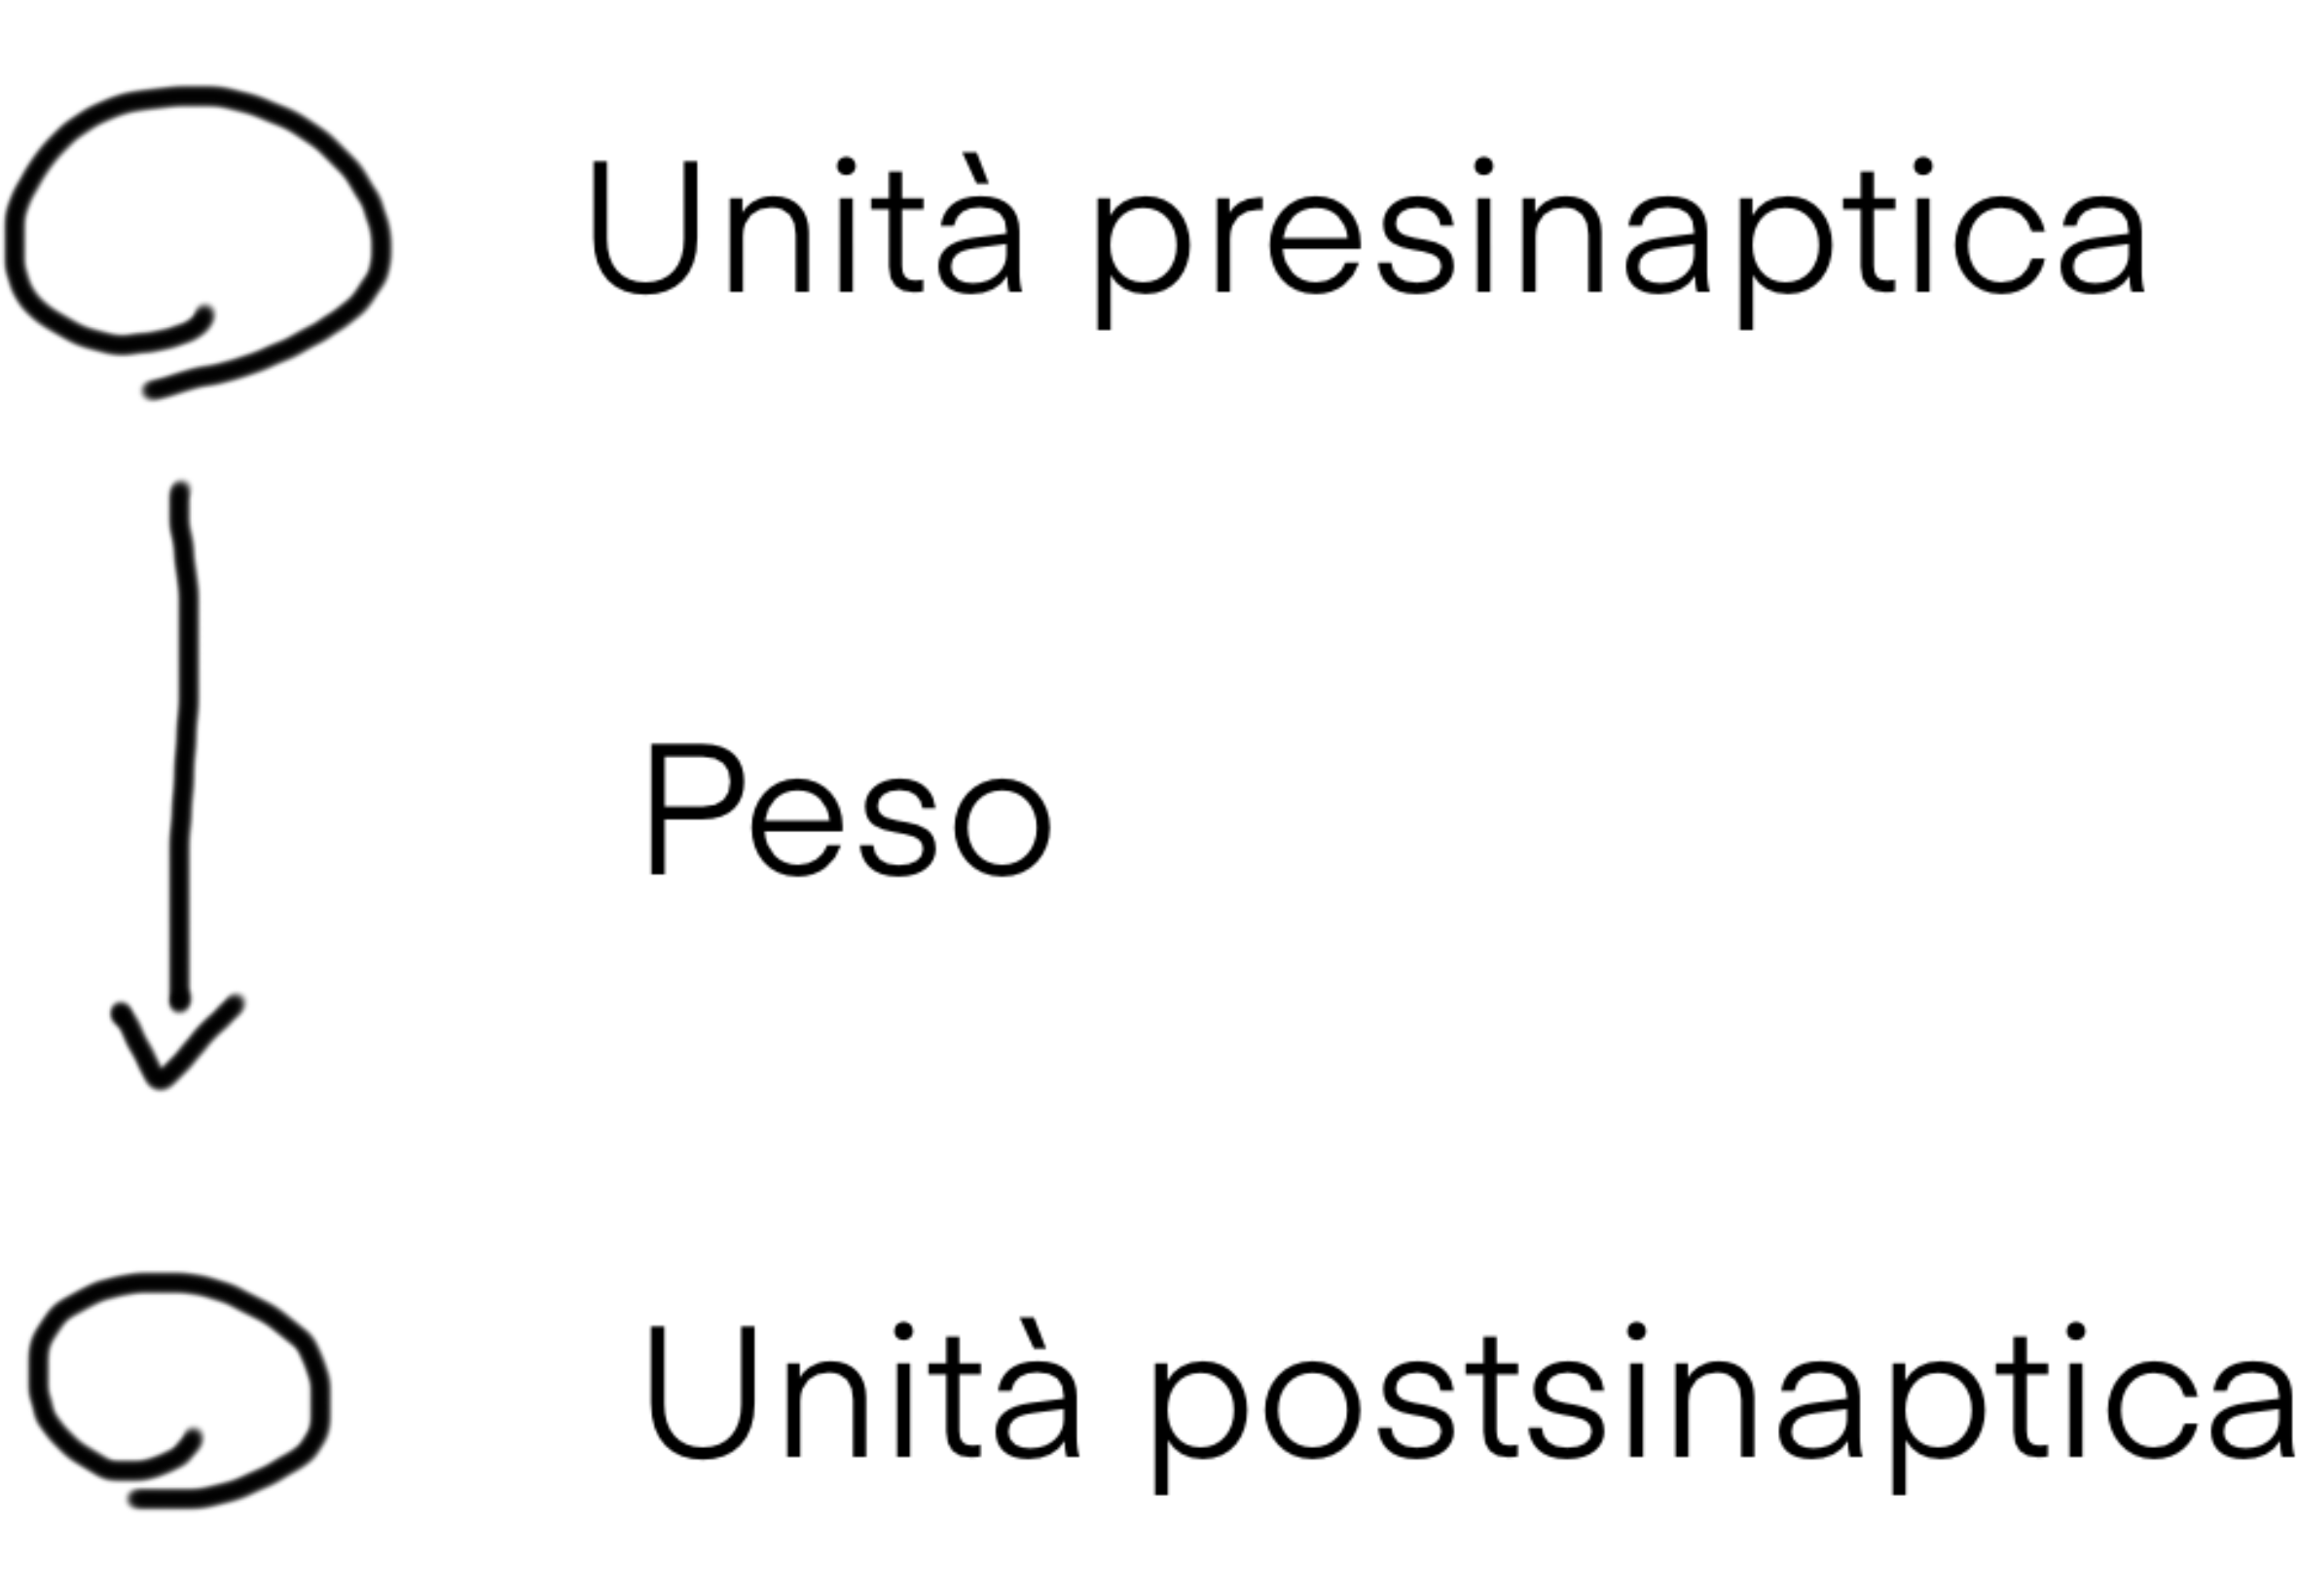
\includegraphics[width=0.3\textwidth]{Hebb}
	\caption{Rete neurale etero-associativa feedforward con un singolo strato di
		sinapsi e con unità binarie.}
\end{figure}

\subsubsection{La regola di Hebb}

Se due neuroni collegati tra di loro sono contemporaneamente attivi, il loro
peso viene incrementato. La regola di Hebb prevede solamente l'incremento dei
pesi, per cui la rete non è in grado di apprendere associazioni che presentano
elementi in comune, ma che richiedono risposte differenti. Dunque la regola di
Hebb permette di apprendere solamente pattern di input che sono ortogonali tra
loro.

\subsubsection{La regola postsinaptica}

Questa regola è anche chiamata regola di Stent-Singer. Il peso viene
incrementato ogni volta che l'unità postsinaptica e l'unità presinaptica sono
entrambe attive; inoltre viene diminuito ogni volta che l'unità postsinaptica è
attiva, ma quella presinaptica è inattiva. Questa regola migliora la generalità,
tuttavia, non fallisce l'apprendimento di pattern di input parzialmente
sovrapposti sullo stesso output, perché tende a creare troppe sinapsi
inibitorie.

\subsubsection{La regola presinaptica}

Il peso viene aumentato quando sia l'unità presinaptica che l'unità
postsinaptica sono attive; il peso viene diminuito quando l'unità presinaptica è
attiva, ma l'unità postsinaptica è inattiva. Questa regola permette di
generalizzare molto meglio rispetto alle regole precedenti.

\subsubsection{La regola della covarianza}

Viene anche chiamata regola di Hopfield. Quando l'unità presinaptica e l'unità
postsinaptica hanno lo stesso stato, il peso viene incrementato; quando hanno
stati opposti, il peso viene diminuito.

\begin{table}[H]
	\centering
	\begin{tabular}{lcccc}
		\hline
		Unità presinaptica  & + & +   & $-$ & $-$ \\
		Unità postsinaptica & + & $-$ & +   & $-$ \\
		\hline
		Hebb                & + &     &     &     \\
		Postsinaptica       & + &     & $-$ &     \\
		Presinaptica        & + & $-$ &     &     \\
		Covarianza          & + & $-$ & $-$ & +   \\
		\hline
	\end{tabular}
	\caption{Riassunto del funzionamento delle regole hebbiane.}
\end{table}

Concludendo, le regole di Hebb possiedono parecchie limitazioni nel tipo di
associazioni che sono in grado di apprendere, poiché sono spesso soggette a
fenomeni di interferenza quando gli input d'ingresso non sono linearmente
indipendenti.


\end{document}
